\begin{enumerate}
\item The ages of two friends ani and Biju differ  by $3$  years. Ani's father dharam is twice as old as Ani and Biju is twice as old as sister cathy. The ages of cathy and dharam differ by $30$ years. Find the ages of Ani and Biju.
\item  One says, \textquotedblleft Give me a hundred, Friend !  I shall then become twice as rich as you \textquotedblright. The other \textquotedblleft  if you give me ten, i shall be six times as rich as you \textquotedblright.  Tell me What is the amount of their (respective) capital? [From the bijaganita of bhaskara II] 
\\ $[Hint: X+100=2(y-100), y+10=6(x-10)]$
\item A train Covered a certain distance at a uniform speed. If the train would have been 10 km/h faster, it would have taken $2$ hours less than the scheduled time. And, if the train were slower by 10 km/h; it would have taken $3$ hours more than the scheduled time. Find the distance covered by the train.
\item The students of a class are made to stand in rows. If 3 Students are extra in a row, there would be $1$ row less. If $3$ students are less in a row, there would be $2$ rows more. Find the number of stuents in the class.
\item In a $\triangle ABC, \angle C=3 \angle B=2(\angle A+\angle B)$. Find the three angles
\item Draw the graphs of the equations $5x-y=5$ and $3x-y=3$. Determine the Co-ordinates of the vertices of the triangle formed by these lines and the $y$ axis.
\item Solve the following pair of linear equations;
\begin{enumerate}
\item
\begin{align}
px+qy=p-q\\ qx-py=p+q
\end{align}
\item
\begin{align}                                                   
ax+by=c\\ bx+ay=1+c
\end{align}
\item 
\begin{align}
\frac {x}{a}-\frac{y}{b}=0\\ ax+by=a^2+b^2
\end{align}
\item
\begin{align}
(a-b)x+(a+b)y=a^2-2ab-b^2\\ (a+b)(x+y)=a^2+b^2
\end{align}
\item
\begin{align}
152x-378y=-74\\ -378x+152y=-604
\end{align}
\end{enumerate}
\item $ABCD$ is a cyclic quadrilateral [see \figref{fig:3.7}]. Find the angles of the cyclic quadrilateral.
\begin{figure}[ht]
\centering
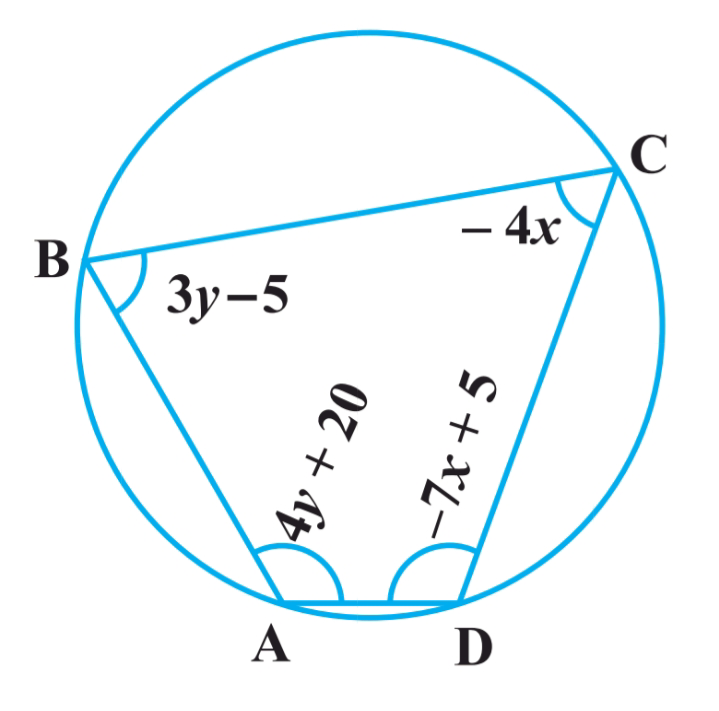
\includegraphics[width=\columnwidth]{chapters/10/figs/3.7.png}
\caption{3.7}
  \label{fig:3.7}
\end{figure}
\end{enumerate}

